\documentclass[aspectratio=169]{beamer}
\usetheme{Madrid}
\usecolortheme{default}
\usepackage{graphicx}
\usepackage{amsmath}
\usepackage{amssymb}
\usepackage{booktabs}
\usepackage{url}




\title[Trustworthy AI: OOD]{Trustworthy Machine Learning: Out-of-Distribution (OOD) Generalization}
\subtitle{Advanced Topics for Data Science in Healthcare}
\author{Chanon Puttanawarut}
\begin{document}

% Slide 1
\begin{frame}
    \titlepage
\end{frame}

% Slide 2
\begin{frame}{Course Outline}
    \tableofcontents
\end{frame}

% Slide 3
\begin{frame}{Reference Material}
    \begin{itemize}
        \item Ji J, Qiu T, Chen B, Zhang B, Lou H, Wang K, et al. AI Alignment: A Comprehensive Survey. arXivOrg 2023. https://arxiv.org/abs/2310.19852v6.
        \item Dalrymple D “davidad,” Skalse J, Bengio Y, Russell S, Tegmark M, Seshia S, et al. Towards Guaranteed Safe AI: A Framework for Ensuring Robust and Reliable AI Systems. arXivOrg 2024. https://arxiv.org/abs/2405.06624v3.
        \item Mucsányi B, Kirchhof M, Nguyen E, Rubinstein A, Oh SJ. Trustworthy Machine Learning 2023.
        \item Liu, Haoyang, Maheep Chaudhary, and Haohan Wang. “Towards Trustworthy and Aligned Machine Learning: A Data-Centric Survey with Causality Perspectives.” arXiv:2307.16851. 


    \end{itemize}
\end{frame}


% Section 1: Introduction & Motivation
\section{Introduction \& Motivation}

\begin{frame}[plain]
    \centering
    \vfill
    {\usebeamerfont{section title}Introduction \& Motivation \par}
    \vfill
  \end{frame}

% Slide 3
\begin{frame}{The Promise of AI}
    \begin{itemize}
        \item Language and image recognition capabilities of AI systems have improved rapidly.
        \item AI systems perform better than humans who did these tests in areas like handwriting recognition, reading comprehension, and image recognition.

    \end{itemize}
    \vspace{-0.3cm}
    \begin{center}
        % TODO: replace with your image file (relative to the project root)
        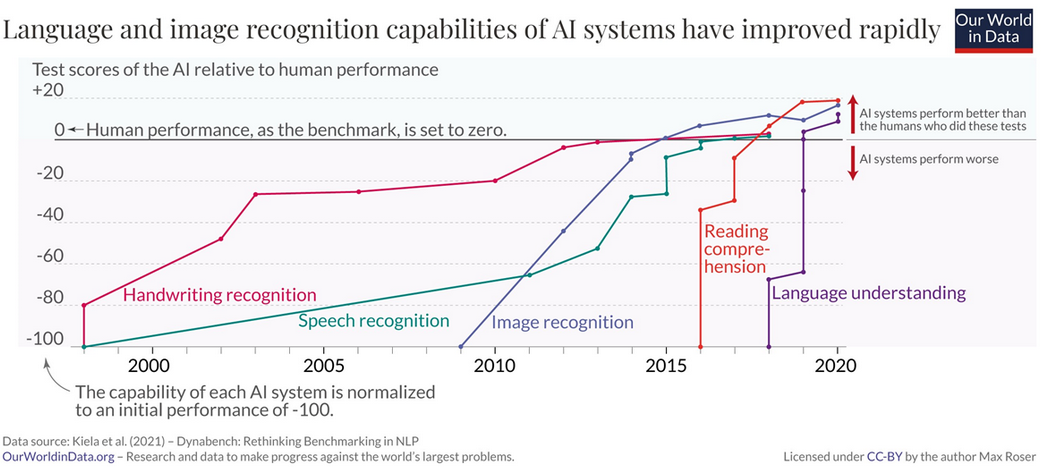
\includegraphics[width=0.75\textwidth]{images/image.png}
    \end{center}
    
\end{frame}

% Slide 4
\begin{frame}{The Human vs. AI Gap: Perspectives from AI Pioneers}
    Despite superhuman test scores on benchmarks, what is current AI still missing?
    \vspace{0.2cm}
    \begin{itemize}
        \item \textbf{Correlation vs. Causation (\textit{Judea Pearl}):} 
        \begin{itemize}
            \item Current ML is highly sophisticated "curve fitting." Humans build causal mental models. AI learns that a chest drain correlates with pneumothorax; a doctor knows it's the \textit{treatment}.
        \end{itemize}
        \item \textbf{Common Sense \& World Models (\textit{Yann LeCun}):} 
        \begin{itemize}
            \item ML requires massive data. Humans learn from a handful of examples because they possess intuitive physics and a "world model" of how reality operates.
        \end{itemize}
        \item \textbf{System 1 vs. System 2 Extrapolation (\textit{Yoshua Bengio}):} 
        \begin{itemize}
            \item AI excels at fast, unconscious pattern matching (System 1). It lacks the slow, conscious reasoning (System 2) required to extrapolate to entirely unseen OOD environments.
        \end{itemize}
        \item \textbf{Underlying World Mechanisms (\textit{Fei-Fei Li}):} 
        \begin{itemize}
            \item AI maps inputs to outputs ($X \rightarrow Y$) without understanding the rich, physical, and contextual reality. Clinical adoption requires AI that understands the actual mechanism of the patient's body, not just pixel patterns.
        \end{itemize}
    \end{itemize}
    \vspace{0.1cm}
    
\end{frame}

% Slide 4
\begin{frame}{Are We Done with ML?}
    Despite high test scores, ML still faces severe limitations:
    \begin{itemize}
        \item \textbf{Dataset constraints:} Data collection is quite expensive, requiring researchers to collect it themselves, use public data, or buy data.
        \item \textbf{Resource constraints:} Hardware and human resources are major bottlenecks.
        \item \textbf{Generalization failure:} Given the same distribution of data, ML models can generalize well. However, if deployed in a new situation (not the same distribution), the model will not work.
    \end{itemize}

\end{frame}



% Slide 5
\begin{frame}{Why Trustworthy AI in Healthcare?}
    When models face shifts at deployment, \emph{mistakes become safety risks}.
    \vspace{0.2cm}
    \begin{itemize}
        \item In healthcare, errors are costly, so we need models that are \textbf{reliable} and \textbf{calibrated} under distribution shift.
        \item If 10 AI systems predict cancer, would you start treatment without a clinician? (We need \textbf{evidence}, not just predictions.)
        \item \textbf{Failure modes} such as hallucinations and spurious correlations severely hinder clinical adoption.
    \end{itemize}
    \vspace{0.3cm}
    
\end{frame}

% Slide 6
\begin{frame}{Core Research Topics in Trustworthy AI}
    \begin{enumerate}
        \item \textbf{Out of distribution (OOD) generalization:} Can we train the model to work well beyond the training distribution?
        \item \textbf{Explainability:} Can we make a model explain itself?
        \item \textbf{Uncertainty:} Can we make a model know when it does not know?
        \item \textbf{Fairness:} Dealing with demographic disparity and use of sensitive attributes.
        \item \textbf{Privacy and security:} How to keep data safe?
        \item \textbf{Causality:} Can we learn cause-and-effect mechanisms rather than correlations?
        \item \textbf{Abuse of AI tools:} Deepfakes and misinformation.
        \item \textbf{Environmental concern:} GPUs consume a lot of energy.
        \item \textbf{Governance and ethics:} Regulation around the use of AI.

        
    \end{enumerate}
\end{frame}



% Slide 8
\begin{frame}{Motivation 1: Pneumothorax Detection}
    \begin{center}
        % TODO: replace with your image file (relative to the project root)
        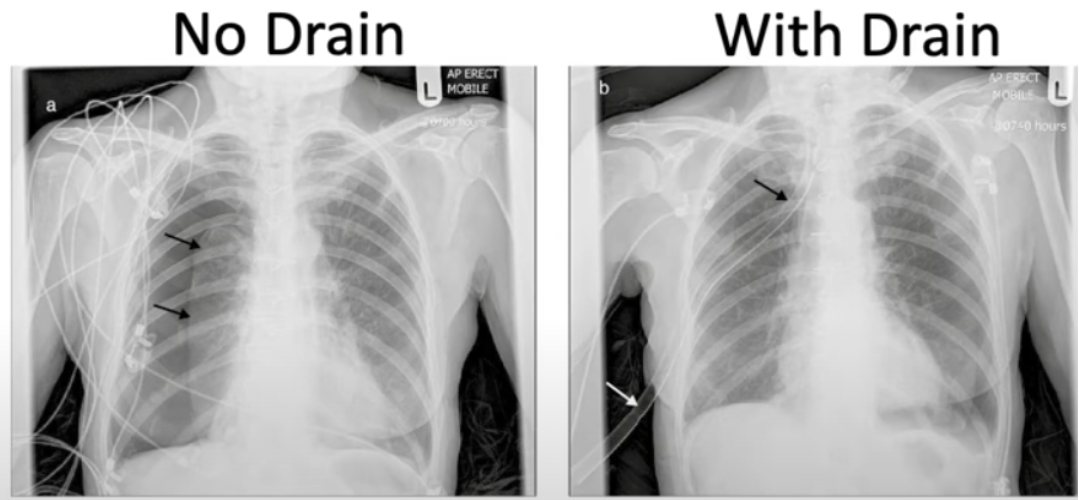
\includegraphics[width=0.60\textwidth]{images/cxr.png}
    \end{center}

    \begin{itemize}
        \item A model for pneumothorax detection achieved an impressive 0.87 AUC.
        \item Performance went down to 0.77 when chest drains were removed from the images.
        \item The model learned to detect the surgical tube, not the underlying lung pathology.
    \end{itemize}

    \scriptsize 

    \url{https://www.youtube.com/watch?v=_4gn7ibByAc}

    \vspace{0.1cm}

    Oakden-Rayner L, Dunnmon J, Carneiro G, Ré C. Hidden stratification causes clinically meaningful failures in machine learning for medical imaging. In Proceedings of the ACM conference on health, inference, and learning 2020 Apr 2 (pp. 151--159).
\end{frame}

% Slide 9
\begin{frame}{Motivation 2: Skin Markings in Dermatology}
    \begin{columns}[T,onlytextwidth]
        \begin{column}{0.5\textwidth}
            \begin{itemize}
                \item There is an association between surgical skin markings in dermoscopic images and the diagnostic performance of deep learning networks for melanoma recognition.
                \item The model exploits the pen marks left by doctors (who suspected cancer) as a predictive feature, ignoring the actual skin lesion.
            \end{itemize}
        \end{column}
        \begin{column}{0.5\textwidth}
            \centering
            % TODO: replace with your image file (relative to the project root)
            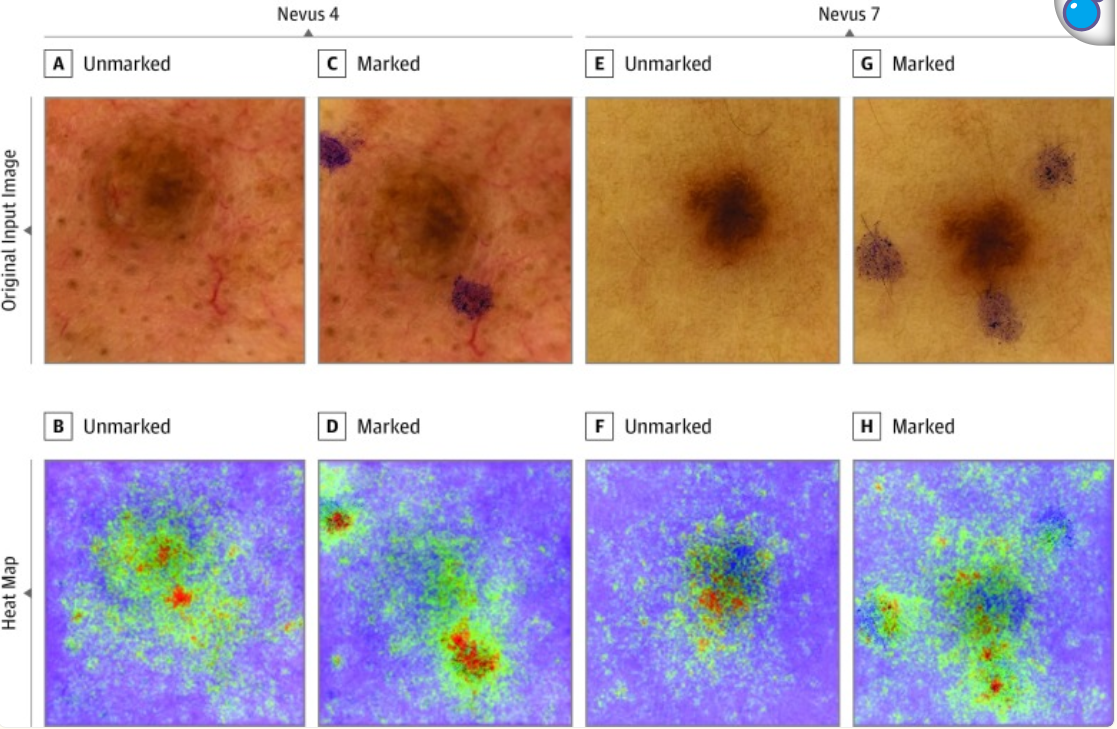
\includegraphics[width=\textwidth]{images/skin.png}
        \end{column}
    \end{columns}
    \vfill
    \scriptsize 


    ref image: Winkler JK, Fink C, Toberer F, Enk A, Deinlein T, Hofmann-Wellenhof R, Thomas L, Lallas A, Blum A, Stolz W, Haenssle HA. Association between surgical skin markings in dermoscopic images and diagnostic performance of a deep learning convolutional neural network for melanoma recognition. JAMA dermatology. 2019 Oct 1;155(10):1135-41.
\end{frame}

% Slide 10
\begin{frame}{Motivation 3: Demographic Bias}
    \begin{columns}[T,onlytextwidth]
        \begin{column}{0.55\textwidth}
            \begin{itemize}
                \item \textbf{Systematic measurement bias:} Pulse oximetry ($SpO_2$) can \emph{overestimate} arterial oxygen saturation ($SaO_2$) in Black patients, with lower discriminative performance (AUC 0.84 vs. 0.89).
                \item \textbf{Higher occult hypoxemia:} In the 92--96\% $SpO_2$ range, Black patients had nearly triple the rate of ``hidden'' hypoxemia ($SaO_2 < 88\%$) vs. White patients (17.0\% vs. 6.2\%).
            \end{itemize}

            \scriptsize Sjoding MW, Dickson RP, Iwashyna TJ, Gay SE, Valley TS. Racial bias in pulse oximetry measurement. New England Journal of Medicine. 2020 Dec 17;383(25):2477-8.
        \end{column}
        \begin{column}{0.45\textwidth}
            \centering
            \small \textit{In the figure:} $Y$ is the true label, and $Z$ is the model prediction.
            % TODO: replace with your image file (relative to the project root)
            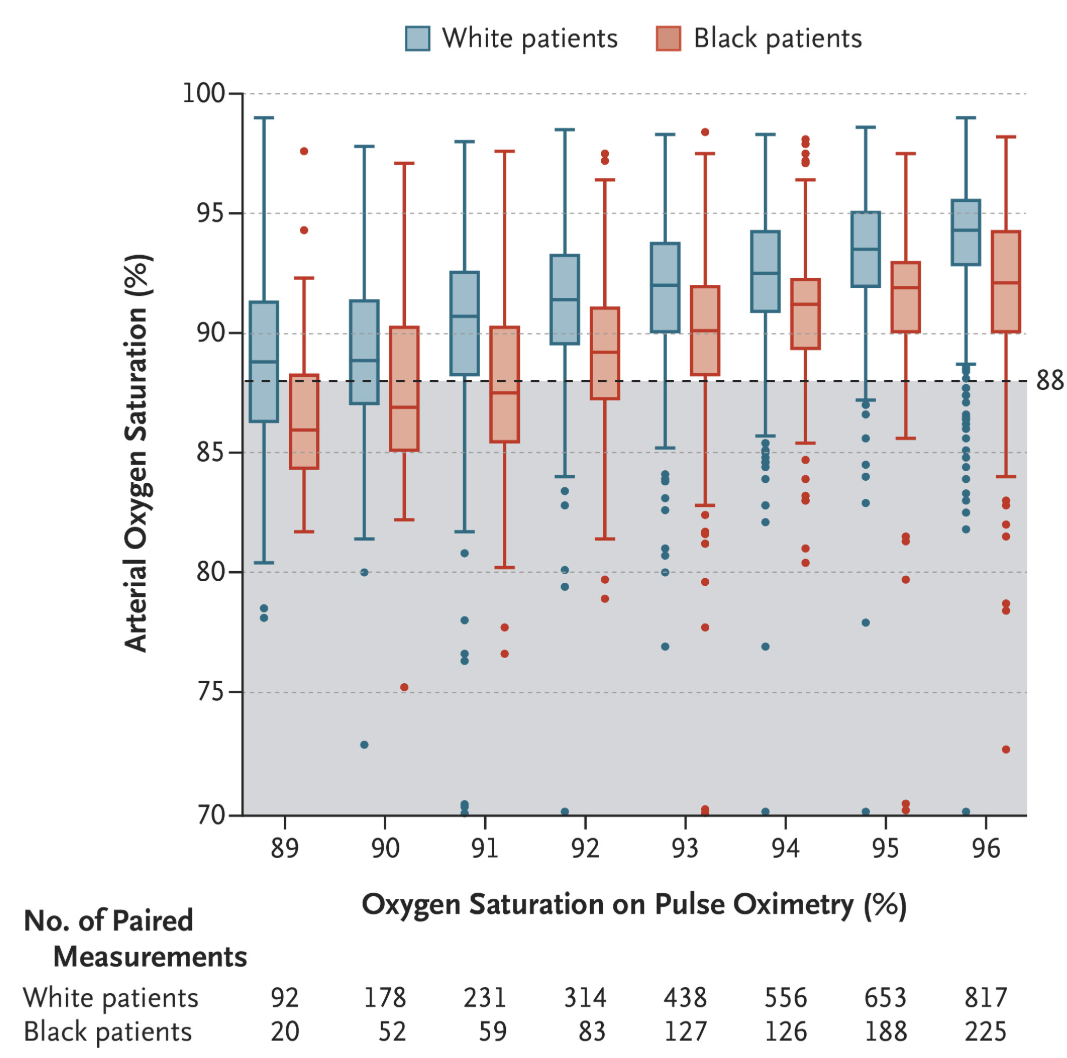
\includegraphics[width=\textwidth]{images/fairness_pulse.png}
        \end{column}
    \end{columns}
\end{frame}



% Section 2: Core Concepts of Generalization
\section{OOD Core Concepts}

\begin{frame}[plain]
    \centering
    \vfill
    {\usebeamerfont{section title}OOD Core Concepts \par}
    \vfill
  \end{frame}

% Slide 11
\begin{frame}{The "What" vs. The "How"}
    \begin{itemize}
        \item Solving "What" (predicting label Y from input X) is not enough.
        \item We must address the "how" part of the problem.
        \item Example: If the label Y is "Car", does the model learn the car body, or does it learn the road (Recognition cue Z)?

    \end{itemize}
    \vspace{0.3cm}
    
\end{frame}




% Slide 11a
\begin{frame}{Example: Same Task, Different Cues (1/3)}
    \centering
    \small A model might rely on the \textit{background} (cue) instead of the object itself (task).
    \vspace{0.2cm}

    % TODO: replace with your image file (relative to the project root)
    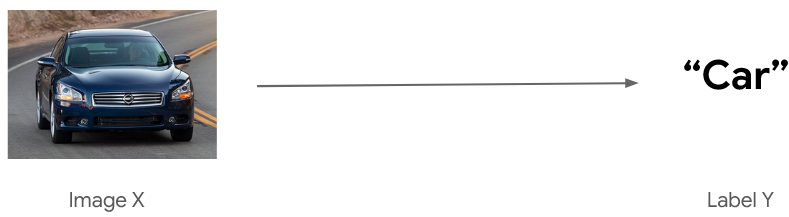
\includegraphics[width=0.85\textwidth]{images/car.png}
\end{frame}

% Slide 11b
\begin{frame}{Example: Same Task, Different Cues (2/3)}
    \centering
    \small If the cue changes at deployment, accuracy can drop even when the task is unchanged.
    \vspace{0.2cm}

    % TODO: replace with your image file (relative to the project root)
    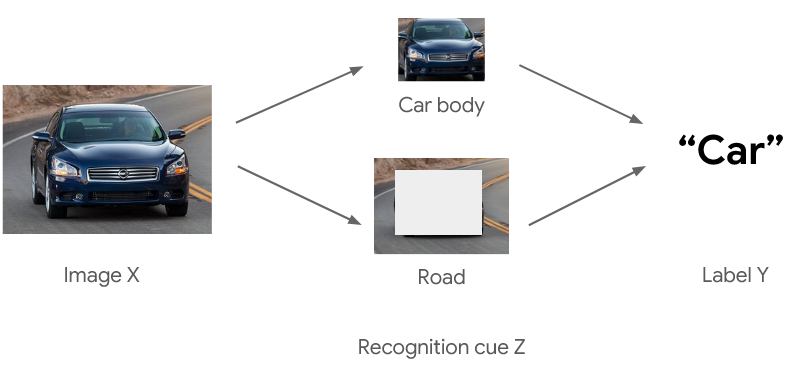
\includegraphics[width=0.85\textwidth]{images/car1.png}
\end{frame}

% Slide 11c
\begin{frame}{Example: Same Task, Different Cues (3/3)}
    \centering
    \small You dont know whether the model learn "Road" or "Car". 
    \vspace{0.2cm}

    % TODO: replace with your image file (relative to the project root)
    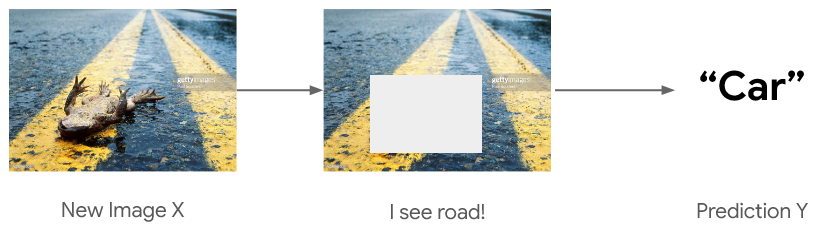
\includegraphics[width=0.85\textwidth]{images/car2.png}
\end{frame}

% Slide 11d (image-only)
\begin{frame}{Chain of thought}
    \centering
    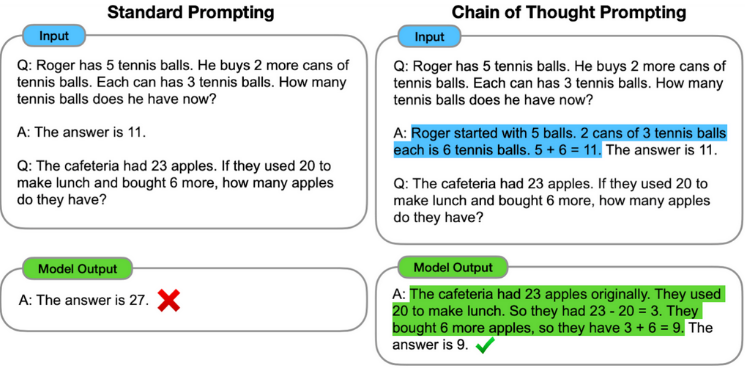
\includegraphics[width=\textwidth,height=\textheight,keepaspectratio]{images/how_LLM.png}
\end{frame}


% Slide 12
\begin{frame}{Terminology: Cues, Tasks, and Domains}
    \begin{itemize}
        \item \textbf{Cue/Feature:} Any factor of variation within data. Cues are inherent to the data.
        \item \textbf{Task:} The factor of variation that matters for you; the factor that you need to recognize at deployment.
        \item Tasks are not inherent to the data; they need to be defined by a human.
        \item \textbf{Domains:} Refers to the environments or sources from which the data originates.
    \end{itemize}

\end{frame}

% Slide 12a (image-only)
\begin{frame}{Cue / Feature (Visualization)}
    \centering
    % TODO: replace with your image file (relative to the project root)
    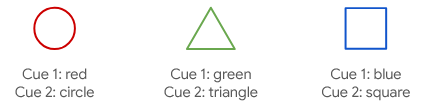
\includegraphics[width=\textwidth,height=0.85\textheight,keepaspectratio]{images/cue.png}
    \scriptsize 
\end{frame}

% Slide 12b (image-only)
\begin{frame}{Task (Visualization)}
    \centering
    % TODO: replace with your image file (relative to the project root)
    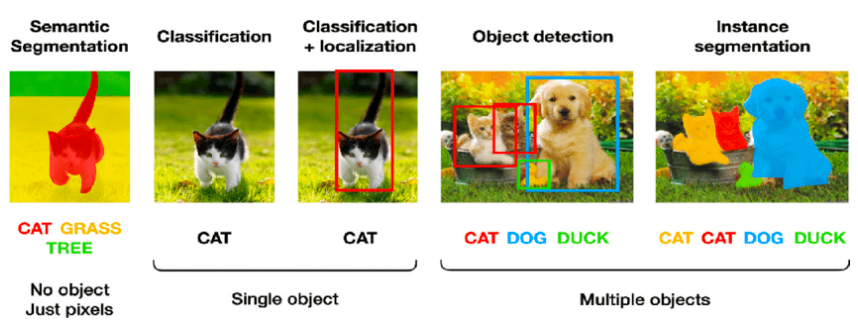
\includegraphics[width=\textwidth,height=0.85\textheight,keepaspectratio]{images/task.png}
    
    \scriptsize
    \url{https://www.researchgate.net/figure/Computer-vision-tasks-Adapted-from_fig5_346091812}
\end{frame}

% Slide 12c (image-only)
\begin{frame}{Domain (Visualization)}
    \centering
    % TODO: replace with your image file (relative to the project root)
    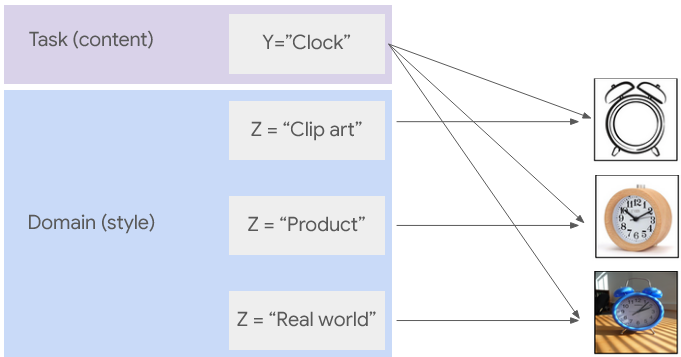
\includegraphics[width=\textwidth,height=0.85\textheight,keepaspectratio]{images/domain.png}
\end{frame}


% Slide 13a
\begin{frame}{Spurious Correlations}
    \begin{columns}[T,onlytextwidth]
        \begin{column}{0.48\textwidth}
            \begin{itemize}
                \item \textbf{Spurious Correlation:} The co-occurrence of cues/features/labels in development data that may not hold at deployment.
                \item A model can appear accurate by exploiting these non-causal cues.
                \item When the correlation breaks, performance drops sharply (OOD failure).
            \end{itemize}
        \end{column}
        \begin{column}{0.5\textwidth}

            \small \textit{In the figure:} $Y$ is the true label, and $Z$ is the model prediction.
            % TODO: replace with your image file (relative to the project root)
            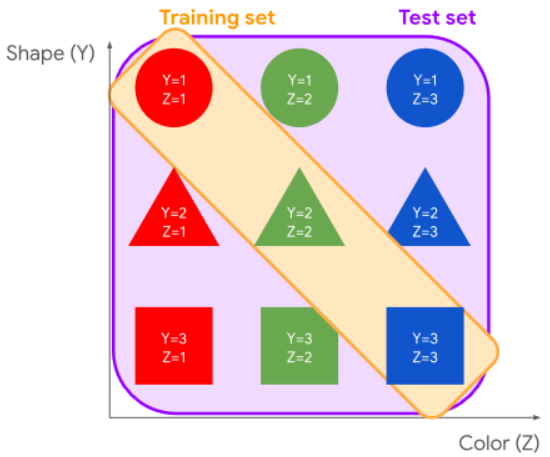
\includegraphics[width=\textwidth]{images/dif.png}
        \end{column}
    \end{columns}
\end{frame}

% Slide 13b
\begin{frame}{Shortcut Learning}
    \begin{itemize}
        \item \textbf{Shortcut Bias:} Models have an inborn preference for "simpler" cues that are predictive in the training set.
        \item The model may choose an easier cue to achieve high training accuracy in an underspecified setting.
        \item Deep networks are often biased toward textures because they can be easier to learn than global shapes.
    \end{itemize}
    
\end{frame}

% Slide 13c
\begin{frame}{Shortcut Learning: Context bias example}
    \begin{center}
        % TODO: replace with your image file (relative to the project root)
        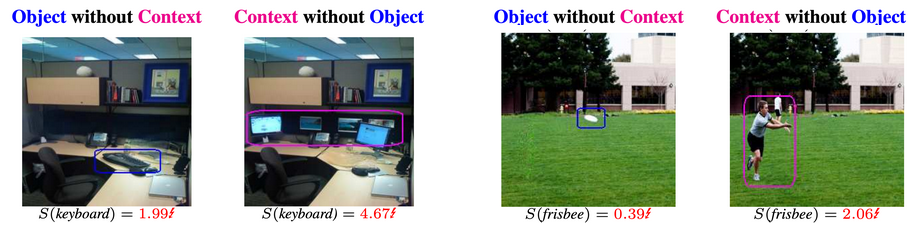
\includegraphics[width=1\textwidth]{images/bias.png}
    \end{center}

    The task cues are the foreground objects, but a classifier focusing on the background context bias cues can achieve high accuracy when the background is highly correlated with the foreground.

    \vspace{0.2cm}

    \scriptsize Not Using the Car to See the Sidewalk — Quantifying and Controlling the Effects of Context in Classification and Segmentation. CVPR 2019.
    
\end{frame}

% Slide 13d
\begin{frame}{Shortcut Learning: Texture bias example}
    \begin{center}
        % TODO: replace with your image file (relative to the project root)
        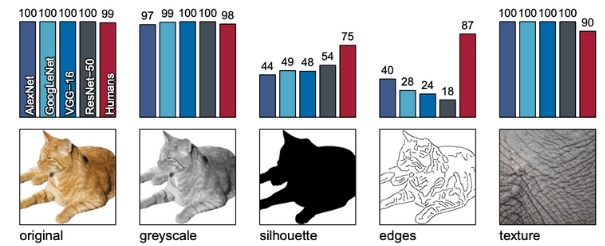
\includegraphics[width=0.8\textwidth]{images/bias2.png}
    \end{center}

    Training a cat/dog classifier on a diagonal dataset, where the texture and shape are highly correlated. At test time, we want to predict cats when changing their texture (e.g., to greyscale, silhouette, edges, or to a marginally different texture).

    \vspace{0.2cm}

    \scriptsize ImageNet-trained CNNs are biased towards texture; increasing shape bias improves accuracy and robustness. ICLR 2019.
\end{frame}





% Slide 14
\begin{frame}{Fairness as a Feature Selection Problem}
    \begin{itemize}
        \item In the context of equality of opportunity, individual fairness dictates that people who are similar with respect to a task should be treated similarly.
        \item Decision makers should avoid differential treatment based on attributes irrelevant to the task.
        \item \textbf{Task Cues:} Features directly relevant and causally linked to the task.
        \item \textbf{Bias Cues:} Features correlated with the task but not causally relevant (e.g., demographic attributes).
    \end{itemize}

\end{frame}

% Slide 15
\begin{frame}{What is OOD Generalization?}
    \textbf{Generalization Types:}
    \begin{table}[]
        \centering
        \setlength{\tabcolsep}{3pt}
        \renewcommand{\arraystretch}{0.9}
        \begin{tabular}{l l l p{4.3cm}}
            \toprule
            \textbf{Generalization Type} & \textbf{How is train=test?} & \textbf{How is train$\neq$test?} & \textbf{Example} \\
            \midrule
            IID & Same distribution & Different samples & Recognise person A whom you see always at office. \\
            OOD Cross-domain & Same task & Different domain & Recognise person A for the first time in a party costume. \\
            OOD Cross-bias & Same task & Different correlation & Recognise person A in person B's jacket. \\
            OOD Adversarial & Same task & Worst-case mismatch & Recognise person A even when A hides identity (e.g., face mask). \\
            \bottomrule
        \end{tabular}
    \end{table}
\end{frame}

% Slide 15a (image-only)
\begin{frame}{OOD Generalization: Cross-Domain}
    \begin{columns}[T,onlytextwidth]
        \begin{column}{0.72\textwidth}
            \centering
            % TODO: replace with your image file (relative to the project root)
            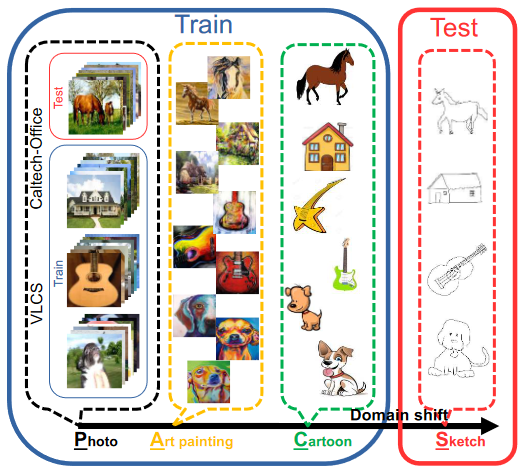
\includegraphics[width=\textwidth,height=0.85\textheight,keepaspectratio]{images/dg_bench.png}
        \end{column}
        \begin{column}{0.28\textwidth}
            \raggedright
            \small Cross-domain generalization: the deployment environment contains completely unseen cues in dev.
        \end{column}
    \end{columns}
\end{frame}

% Slide 15b (image-only)
\begin{frame}{OOD Generalization: Cross-Bias}
    \begin{columns}[T,onlytextwidth]
        \begin{column}{0.72\textwidth}
            \centering
            % TODO: replace with your image file (relative to the project root)
            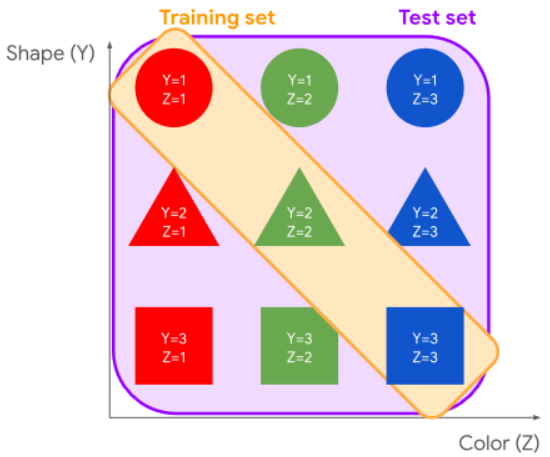
\includegraphics[width=\textwidth,height=0.85\textheight,keepaspectratio]{images/dif.png}
        \end{column}
        \begin{column}{0.28\textwidth}
            \raggedright
            \small Cross-bias generalization: deployment contains unseen compositions of seen cues in dev.
        \end{column}
    \end{columns}
\end{frame}



% Slide: Why OOD Generalization? (1/3)
\begin{frame}{Why Do We Need OOD Generalization? (1/3)}
    \begin{center}
        % TODO: replace with your image file (relative to the project root)
        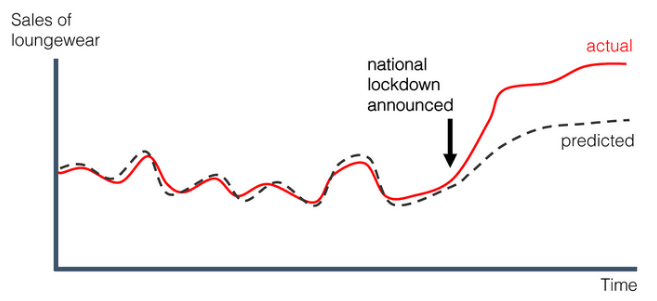
\includegraphics[width=0.85\textwidth]{images/reason_ood.png}
    \end{center}

    \begin{itemize}
        \item \textbf{COVID-19 lockdowns caused abrupt distribution shift:} patient mix, care-seeking behavior, and clinical workflows changed.
.
    \end{itemize}

\end{frame}

% Slide: Why OOD Generalization? (2/3)
\begin{frame}{Why Do We Need OOD Generalization? (2/3)}


    \begin{itemize}
        \item \textbf{Model decay (concept drift):} performance can degrade over time as practice patterns, devices, and populations evolve.
        \item \textbf{Retraining helps, but is not free:} needs monitoring, fresh labels, validation, and governance to avoid regressions.

    \end{itemize}
    \vspace{0.2cm}
    \begin{center}
        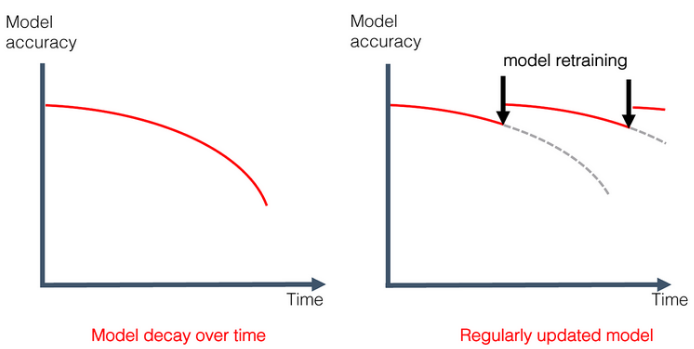
\includegraphics[width=0.75\textwidth]{images/reason_ood2.png}
    \end{center}
\end{frame}

% Slide: Why OOD Generalization? (3/3)
\begin{frame}{Why Do We Need OOD Generalization? (3/3)}
    \begin{center}
        % TODO: replace with your image file (relative to the project root)
        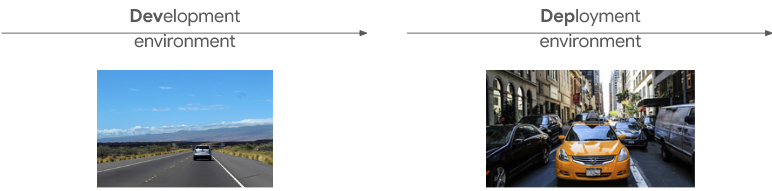
\includegraphics[width=1\textwidth]{images/ood.png}
    \end{center}

    \begin{itemize}
        \item \textbf{Development environment $\neq$ deployment environment:} training data is curated; deployment data is messy.

    \end{itemize}

\end{frame}

% Slide 16
\begin{frame}{Mathematical Framing of OOD}
    Let $\mathcal{D}_{tr} = \{(x_i, y_i)\}_{i=1}^N \sim P_{dev}(X,Y)$ be our development set. \\
    Let $P_{deploy}(X,Y)$ be the unseen deployment distribution.
    \vspace{0.5cm}
    \begin{itemize}
        \item \textbf{IID Assumption:} $P_{dev}(X,Y) = P_{deploy}(X,Y)$
        \item \textbf{OOD Setting:} $P_{dev}(X,Y) \neq P_{deploy}(X,Y)$
    \end{itemize}
    \vspace{0.5cm}
    Our goal is to learn parameters $\theta$ that minimize the expected risk on the deployment distribution:
    $$ \min_{\theta} \mathbb{E}_{(x,y) \sim P_{deploy}} [\ell(f_\theta(x), y)] $$
    Without access to $P_{deploy}$, standard empirical risk minimization (ERM) on $\mathcal{D}_{tr}$ fails.
\end{frame}

% Section 3: Development, Deployment, and Leakage
\section{Development, Deployment, and Evaluation Traps}

% Slide 17
\begin{frame}{Development vs. Deployment Stages}
    Simulating a real world ML setting involves strict data splits:
    \begin{itemize}
        \item \textbf{Train:} Development samples where the model parameters are updated.
        \item \textbf{Val:} Development samples on which hyperparameters and discrete design choices are made.
        \item \textbf{Test:} Testing is a lab setup designed to mimic the deployment scenario closely.
    \end{itemize}
    \vspace{0.2cm}
    Academia view: The test set and the action of testing is treated as a part of the deployment. ML becomes arbitrarily easier if information from the deployment stage is available during development.
\end{frame}

% Slide 18
\begin{frame}{The Information Leakage Paradox}
    \begin{itemize}
        \item It is common to evaluate models on labeled samples from a target domain to measure performance.
        \item However, as soon as we use target domain for evaluation, we are no longer strictly in a domain generalization setting, since the model has interacted with the target domain.
        \item Evaluating domain generalization models on benchmarks is paradoxical, as it often involves repeated observations of the target domain.
        \item \textbf{Solutions:} Select hyperparameters using development resources and minimize use of the test set.
    \end{itemize}

    \begin{columns}[T,onlytextwidth]
        \begin{column}{0.49\textwidth}
            \centering
            % TODO: replace with your left image file (relative to the project root)
            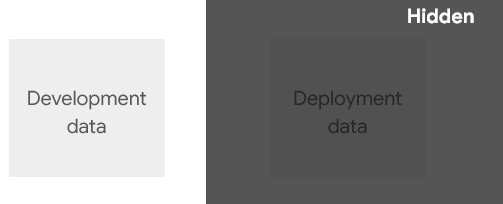
\includegraphics[width=\textwidth]{images/paradox.png}
        \end{column}
        \begin{column}{0.49\textwidth}
            \centering
            % TODO: replace with your right image file (relative to the project root)
            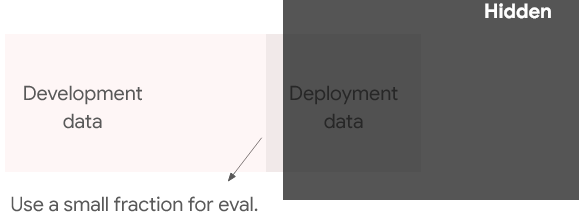
\includegraphics[width=\textwidth]{images/paradox2.png}
        \end{column}
    \end{columns}
\end{frame}


% Slide 19
\begin{frame}{Similar topic to OOD}
\textbf{Common settings related/similar to OOD generalization}
\vspace{0.2cm}

\begin{columns}[T,onlytextwidth]
    \begin{column}{0.53\textwidth}
        \textbf{Different domain/distribution settings}
        \begin{itemize}
            \item In-Distribution (ID) generalization
            \item Out-of-Distribution (OOD) generalization
            \item Domain adaptation
            \item Domain generalisation
            \item Test-time training
            \item Continual learning
        \end{itemize}
    \end{column}
    \begin{column}{0.47\textwidth}
        \textbf{Different task settings}
        \begin{itemize}
            \item Transfer learning
            \item $k$-shot learning
            \item Meta-learning
            \item Continual learning
        \end{itemize}
    \end{column}
\end{columns}
\end{frame}

% Slides: Different settings (insert after "How to Achieve OOD Generalization?")
% Different Domain/Distribution Settings
\begin{frame}{Different Domain/Distribution Settings: In-Distribution (ID) Generalization}
    \begin{itemize}
        \item \textbf{Goal:} Generalize to new samples drawn from the \emph{same} distribution as training.
        \item \textbf{Assumption:} $P_{train}(X,Y) \approx P_{test}(X,Y)$ (IID).
        \item \textbf{Example (healthcare):} Same hospital, same scanner, same protocol; new patients.
    \end{itemize}

    \begin{center}
        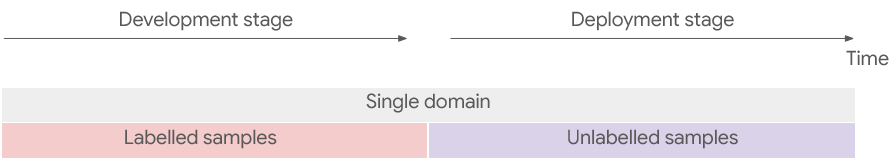
\includegraphics[width=1\textwidth]{images/id_gen.png}
    \end{center}
\end{frame}

\begin{frame}{Different Domain/Distribution Settings: Out-of-Distribution (OOD) Generalization}
    \begin{itemize}
        \item \textbf{Goal:} Maintain performance when the deployment distribution shifts.
        \item \textbf{Assumption:} $P_{train}(X,Y) \neq P_{test}(X,Y)$, but the \emph{task} is the same.
        \item \textbf{Example:} Train on Hospital A CXR; deploy on Hospital B with different devices/population.
    \end{itemize}

    \begin{center}
        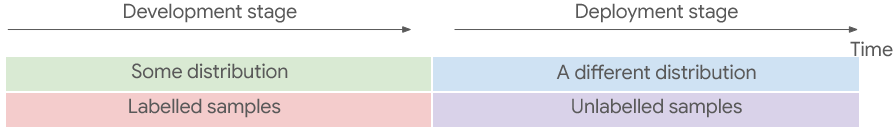
\includegraphics[width=0.99\textwidth]{images/ood_gen.png}
    \end{center}
\end{frame}

\begin{frame}{Different Domain/Distribution Settings: Domain Adaptation}
    \begin{itemize}
        \item \textbf{Goal:} Adapt a model to a \emph{specific} target domain.
        \item \textbf{Key resource:} Access to target-domain data during development (labeled or unlabeled).
        \item \textbf{Example:} Unlabeled target CXRs used to align feature distributions before deployment.
    \end{itemize}
    \vspace{0.2cm}
    \begin{center}
        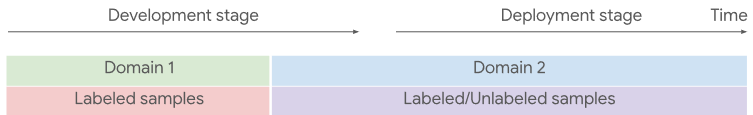
\includegraphics[width=0.999\textwidth]{images/da.png}
    \end{center}
\end{frame}

\begin{frame}{Different Domain/Distribution Settings: Domain Generalisation}
    \begin{itemize}
        \item \textbf{Goal:} Train on multiple source domains and perform well on an \emph{unseen} domain.
        \item \textbf{Constraint:} No access to the target domain during training/validation.
        \item \textbf{Example:} Train on multiple hospitals; deploy to a new hospital with no target samples.
    \end{itemize}
    \vspace{0.2cm}
    \begin{center}
        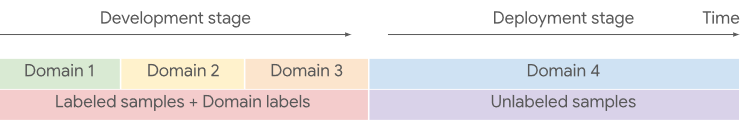
\includegraphics[width=0.999\textwidth]{images/dg.png}
    \end{center}
\end{frame}

\begin{frame}{Different Domain/Distribution Settings: Test-time Training}
    \begin{itemize}
        \item \textbf{Goal:} Improve robustness by updating the model \emph{at deployment time}.
        \item \textbf{Typical setup:} Use unlabeled test samples with a self-supervised or entropy objective.
        \item \textbf{Example:} Update batch-norm / minimize prediction entropy on incoming CXRs.
    \end{itemize}
    \vspace{0.2cm}
    \begin{center}
        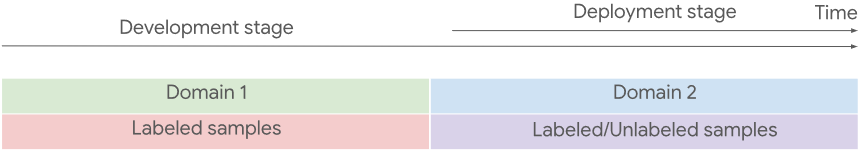
\includegraphics[width=0.999\textwidth]{images/ttt.png}
    \end{center}
\end{frame}

\begin{frame}{Different Domain/Distribution Settings: Continual Learning}
    \begin{itemize}
        \item \textbf{Goal:} Learn from a stream of changing data/tasks without catastrophic forgetting.
        \item \textbf{Challenge:} New domains over time + limited access to past data.
        \item \textbf{Example:} Model updated across months/years as scanners/protocols/patient mix evolve.
    \end{itemize}
    \vspace{0.2cm}
    \begin{center}
        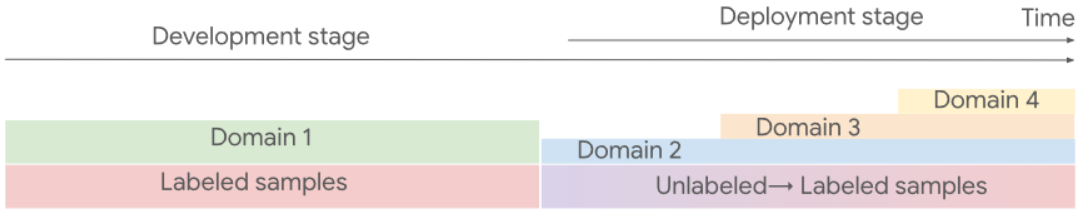
\includegraphics[width=0.999\textwidth]{images/cl.png}
    \end{center}
\end{frame}

% Different Task Settings
\begin{frame}{Different Task Settings: Transfer Learning}
    \begin{itemize}
        \item \textbf{Goal:} Reuse representations learned on a source task/domain for a target task.
        \item \textbf{Typical recipe:} Pretrain (e.g., ImageNet / large medical dataset) $\rightarrow$ fine-tune.
        \item \textbf{When useful:} Target labels are scarce; faster convergence and better accuracy.
    \end{itemize}
    \vspace{0.2cm}
    \begin{center}
        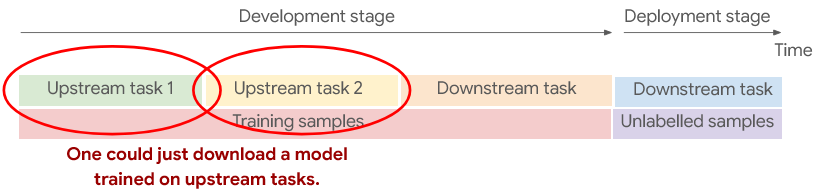
\includegraphics[width=0.75\textwidth]{images/tl.png}
    \end{center}
\end{frame}

\begin{frame}{Different Task Settings: K-shot Learning}
    \begin{itemize}
        \item \textbf{Goal:} Learn a new task/class from $k$ labeled examples (few-shot).
        \item \textbf{Key challenge:} Avoid overfitting when $k$ is small (e.g., 1, 5, 10).
        \item \textbf{Example:} Identify a rare disease with only a handful of confirmed labeled cases.
    \end{itemize}
    \vspace{0.2cm}
    \begin{center}
        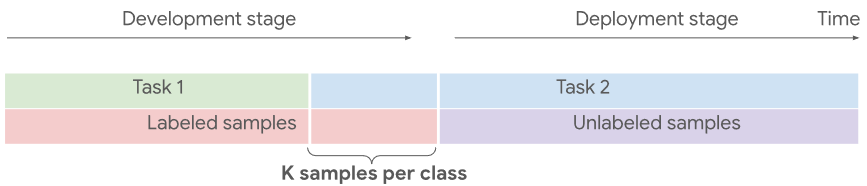
\includegraphics[width=0.999\textwidth]{images/k_shot.png}
    \end{center}
\end{frame}

\begin{frame}{Different Task Settings: Meta-Learning}
    \begin{itemize}
        \item \textbf{Goal:} ``Learn to learn'' across many tasks so adaptation to a new task is fast.
        \item \textbf{Idea:} Optimize for parameters/representations that adapt well with few gradient steps.
        \item \textbf{Example:} Train across many clinical classification tasks to enable rapid new task setup.
    \end{itemize}
    \vspace{0.2cm}
    \begin{center}
        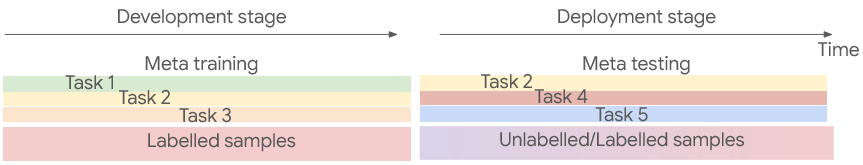
\includegraphics[width=0.999\textwidth]{images/meta.png}
    \end{center}
\end{frame}

\begin{frame}{Different Task Settings: Continual learning}
    \begin{itemize}
        \item \textbf{Goal:} Accumulate capabilities over a sequence of tasks (not just domains).
        \item \textbf{Challenge:} Catastrophic forgetting vs. plasticity to learn new tasks.
        \item \textbf{Example:} Expand from pneumothorax detection to effusion to edema over time.
    \end{itemize}
    \vspace{0.2cm}
    \begin{center}
        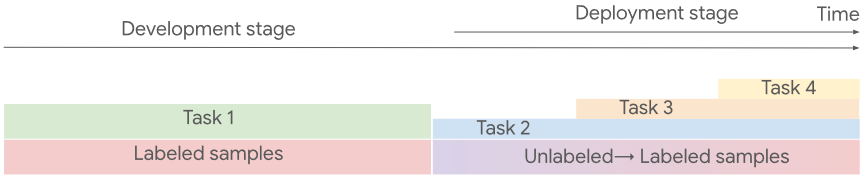
\includegraphics[width=0.999\textwidth]{images/ticl.png}
    \end{center}
\end{frame}

% Section 4: Algorithmic Solutions (Debiasing)
\section{OOD Solutions}

\begin{frame}[plain]
    \centering
    \vfill
    {\usebeamerfont{section title}OOD Solutions \par}
    \vfill
  \end{frame}

\begin{frame}{OOD setting}

    \renewcommand{\arraystretch}{1.25}
    \setlength{\tabcolsep}{6pt}
    \begin{table}
    \centering
    \scriptsize
    \begin{tabular}{p{2.6cm} p{3.3cm} p{3.3cm} p{3.6cm}}
        \toprule
        \textbf{Settings} &
        \textbf{All training samples are biased} &
        \textbf{Some unbiased training samples; no bias label} &
        \textbf{Some unbiased training samples; bias label available} \\
        \midrule
        \textbf{No test samples} &
        \textcolor{red}{Impossible to solve} &
        Detect unbiased samples and put more weights on them &
        Put more weights on unbiased samples \\
        \midrule
        \textbf{A few unlabeled test samples} &
        Train multiple hypotheses and do model selection &
        Combination of methods &
        Combination of methods \\
        \midrule
        \textbf{A few labeled test samples} &
        Train multiple hypotheses and do model selection &
        Combination of methods &
        Combination of methods \\
        \bottomrule
    \end{tabular}
    \end{table}
\end{frame}

% Slide 20
\begin{frame}{Debias (bias label available): Simple Balancing}
    \textbf{Assumption:} We have bias/domain labels (e.g., hospital/site) for each training sample.

    \begin{itemize}
        \item \textbf{Goal:} Reduce spurious correlation by making the training data \emph{less biased} across domains.
        \item \textbf{Simple method:} Re-balance mini-batches so each domain contributes equally.

    \end{itemize}

    \begin{center}
        % TODO: replace with your image file (relative to the project root)
        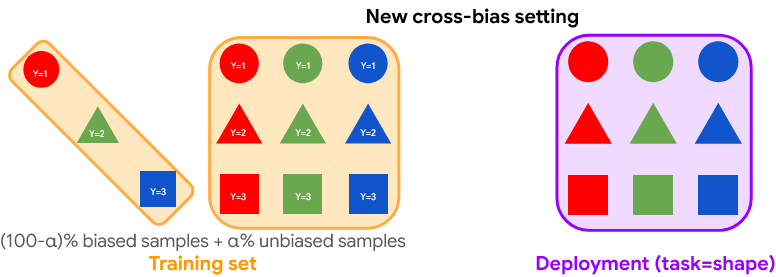
\includegraphics[width=0.85\textwidth]{images/1_weight.png}
    \end{center}

    \scriptsize Idrissi, B. Y., Arjovsky, M., Pezeshki, M., & Lopez-Paz, D. (2021, October 27). Simple data balancing achieves competitive worst-group-accuracy.
\end{frame}

% Slide 21
\begin{frame}{Debias (bias label available): Domain-Adversarial Neural Networks}
    \textbf{Assumption:} We have labels for the bias (e.g., we know which hospital each X-ray comes from).
    \begin{itemize}
        \item \textbf{Concept:} Add an additional head to the model that predicts bias/domain labels.
        \item Adversarially train the feature extractor so the extracted features are maximally noninformative for predicting bias labels.
        \item The features must remain informative for the original head to solve the main task.
    \end{itemize}
    
\end{frame}

% Slide 22
\begin{frame}{Domain-Adversarial Neural Networks}
    Let $G_f(\theta_f)$ be the feature extractor, $G_y(\theta_y)$ the task predictor, and $G_d(\theta_d)$ the domain classifier.
    We jointly optimize:
    $$ \min_{\theta_f, \theta_y} \max_{\theta_d} \mathcal{L}_{task}(\theta_f, \theta_y) - \lambda \mathcal{L}_{domain}(\theta_f, \theta_d) $$
    \vspace{-0.2cm}
    \begin{center}
        % TODO: replace with your image file (relative to the project root)
        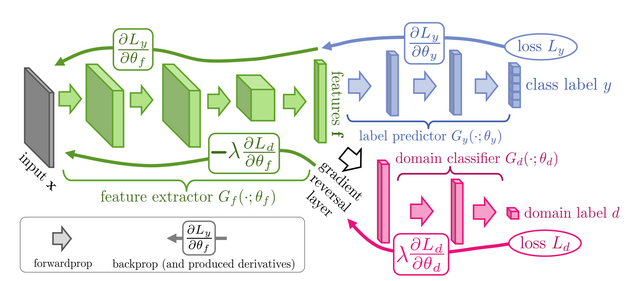
\includegraphics[width=0.7\textwidth]{images/dann.png}
    \end{center}
    \scriptsize Domain-adversarial training of neural networks. JMLR 2016.
\end{frame}

% Slide 23
\begin{frame}{Debias (bias label unavailable): Unknown Bias}

    \textbf{Intuition:} We must make an assumption.
    \begin{itemize}
        \item We know that models possess a shortcut bias favoring simple cues.
        \item Therefore, we assume bias is the \textit{first} cue learned by a generic model.
        \item Bias is the cue learned by a model of limited capacity (e.g., small CNN with small receptive field).
    \end{itemize}

\begin{center}
    % TODO: replace with your image file (relative to the project root)
    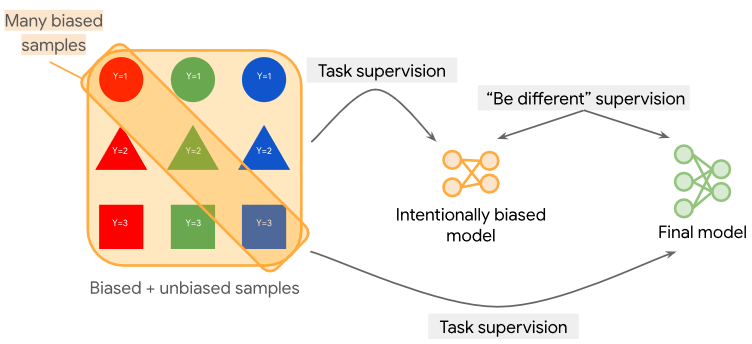
\includegraphics[width=0.7\textwidth]{images/2.png}
\end{center}

\end{frame}

% Slide 23b (two images: left/right)
\begin{frame}{Receptive field}
    \begin{columns}[T,onlytextwidth]
        \column{0.5\textwidth}
        \centering
        % TODO: replace with your image file (relative to the project root)
        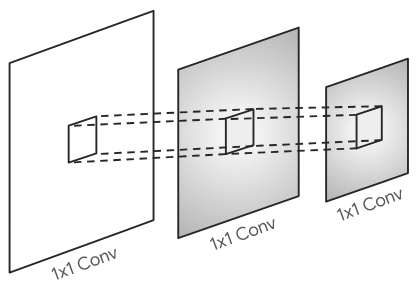
\includegraphics[width=\linewidth]{images/bias3.png}
        
        \column{0.5\textwidth}
        \centering
        % TODO: replace with your image file (relative to the project root)
        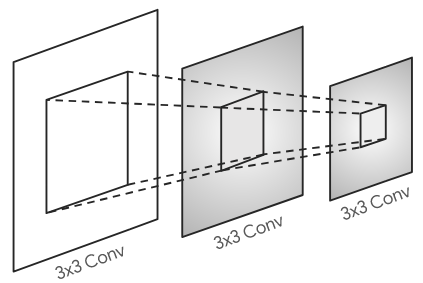
\includegraphics[width=\linewidth]{images/bias4.png}
    \end{columns}
\end{frame}


% Slide 24
\begin{frame}{Learning from Failure (LfF)}
    Learning from Failure (LfF) utilizes "Be Different" supervision: forces a final model to be different from an intentionally biased model.
    \begin{itemize}
        \item \textbf{Intentionally Biased Model $B$:} Train a model constrained to capture local cues.
        \item \textbf{Final Model $D$:} Train a more comprehensive model with loss minimization that reduces similarity to the biased model $B$.
    \end{itemize}
    If $B$ only looks at textures (bias), $D$ is forced to look at shapes (task).

    \vspace{0.2cm}
    \textbf{Re-weighting (key idea):}
    \[
        w(x)=\frac{\mathrm{CE}\!\left(f_{B}(x),y\right)}{\mathrm{CE}\!\left(f_{B}(x),y\right)+\mathrm{CE}\!\left(f_{D}(x),y\right)}
    \]
    \[
        \theta_{D}\leftarrow\theta_{D}-\eta\nabla_{\theta_{D}}\sum_{(x,y)\in\mathcal{B}} w(x)\cdot \mathrm{CE}\!\left(f_{D}(x),y\right)
    \]

    \scriptsize Learning from Failure: Training Debiased Classifier from Biased Classifier. NeurIPS 2020.
\end{frame}

% Slide 25 (picture only)
\begin{frame}[plain]{Learning from Failure (LfF)}
\[
        w(x)=\frac{\mathrm{CE}\!\left(f_{B}(x),y\right)}{\mathrm{CE}\!\left(f_{B}(x),y\right)+\mathrm{CE}\!\left(f_{D}(x),y\right)}
    \]
    \[
        \theta_{D}\leftarrow\theta_{D}-\eta\nabla_{\theta_{D}}\sum_{(x,y)\in\mathcal{B}} w(x)\cdot \mathrm{CE}\!\left(f_{D}(x),y\right)
    \]
    \centering
    % TODO: replace with your image file (relative to the project root)
    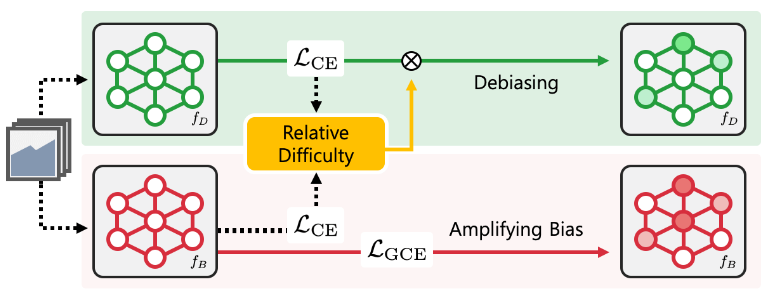
\includegraphics[height=0.6\textheight]{images/2_lff.png}
\end{frame}


% Slide 26
\begin{frame}{ReBias: Removing Bias with Bias}

    \begin{itemize}
        \item \textbf{Concept:} Train a de-biased representation by encouraging it to be statistically independent from representations that are intentionally biased.
        \item \textbf{Intentionally Biased Models $g$:} Models constrained to capture shortcuts, such as small receptive field CNNs for texture bias.
        \item \textbf{Final Model $f$:} Learns the target task while "running away" from the biased models $g$.
        \item \textbf{HSIC:} Uses the Hilbert-Schmidt Independence Criterion to measure and penalize the dependence between the continuous random variables $f(X)$ and $g(X)$.
    \end{itemize}

    \scriptsize Learning De-biased Representations with Biased Representations. ICML 2020
\end{frame}

% Slide 27
\begin{frame}{ReBias: Minimax Optimization}
    \textbf{Objective:} Minimax optimization is used for bias removal.
    \begin{itemize}
        \item The primary model $f$ minimizes the main task loss $\mathcal{L}$ while maximizing independence from the biased models.
        \item The biased model $g \in G$ minimizes its own task loss to intentionally overfit to the bias.
    \end{itemize}

    \[
        \min_{f} \left\{ \mathcal{L}(f) + \lambda \max_{g} \left( \text{HSIC}_1(f, g) - \lambda_g \mathcal{L}(g) \right) \right\}
    \]
   
    
    \begin{center}
        % TODO: replace with your image file (relative to the project root)
        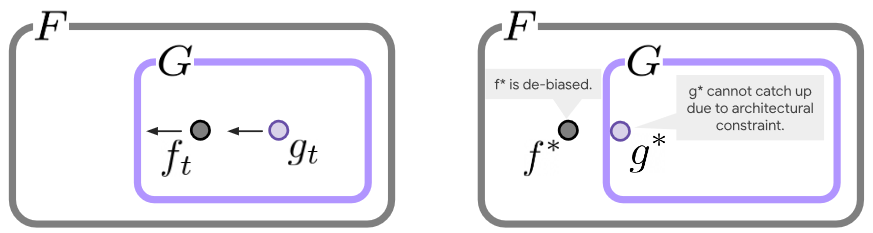
\includegraphics[height=0.45\textheight]{images/3_rebias5.png}
    \end{center}
    
    \scriptsize Learning De-biased Representations with Biased Representations. ICML 2020.
\end{frame}


% Slide 33
\begin{frame}{Course Summary}
    \begin{itemize}
        \item \textbf{Goal:} Build \textit{trustworthy} ML systems that remain reliable under \textbf{distribution shift}.
        \item \textbf{Core problem:} ERM learns correlations that can break OOD; real deployments involve domain shift, label shift, and spurious shortcuts.
        \item \textbf{How we evaluate trust:} separate in-distribution vs.\ OOD test sets, calibration/uncertainty, and stress tests for failure modes.
        \item \textbf{Key strategies covered:}
        \begin{itemize}
            \item \textit{Data-centric:} improve coverage, reduce dataset bias, and use re-weighting/augmentation.
            \item \textit{Robust learning:} invariance/regularization and methods that discourage shortcut features.
            \item \textit{Deployment:} monitor shift, validate continually, and keep humans-in-the-loop for safety-critical decisions.
        \end{itemize}
        \item \textbf{Takeaway:} Trustworthiness is not a single metric---it is a \textbf{pipeline} from data to evaluation to monitoring.
    \end{itemize}
\end{frame}

\begin{frame}
    \begin{center}
        \Huge \textbf{Thank You!} \\
        \vspace{1cm}
        \Large Questions?
    \end{center}
\end{frame}

\end{document}